
\begin{center}
\textbf{\large 4. ВЛИЯНИЕ ДАЛЬНОДЕЙСТВИЯ СИЛЫ ПРИТЯЖЕНИЯ НА СКОРОСТЬ НУКЛЕАЦИИ}
\end{center}
\refstepcounter{chapter}
\addcontentsline{toc}{chapter}{4. ВЛИЯНИЕ ДАЛЬНОДЕЙСТВИЯ СИЛЫ ПРИТЯЖЕНИЯ НА СКОРОСТЬ НУКЛЕАЦИИ}

\section{Введение}
\label{PRIMe-SecIntroduction}

Построение фазовых диаграмм различных систем является крайне важным для многих направлений науки и техники.
На данный момент удобным инструментом для изучения фазовых состояний веществ на уровне отдельных частиц является метод молекулярной динамики~\cite{10.1063/1.1730376, 10.1006/jcph.1995.1039} и модельных систем.
Примером служат пылевая плазма и коллойдные частицы во вращающихся электрических и магнитных полях~\cite{10.1038/s41598-017-14001-y, 10.1103/physreve.103.022608, 10.1103/physreve.96.043201}.
Для построения фазовых диаграмм систем существует несколько способов расчета, которые основаны на знании координат частиц в каждый момент времени.
К ним относятся термодинамическое интегрирование~\cite{10.1088/0953-8984/21/46/465104}, кластеризация с помощью разбиения на ячейки Вороного~\cite{10.1021/acs.jpcc.7b09317} и метод вычисления плотности газа и конденсата с помощью расчета профиля плотности системы с зафиксированными в пространстве газовой и конденсированной фазами~\cite{10.1021/jp806127j, 10.1021/jp1117213}.

Однако каждый из этих методов имеет ряд недостатков, которые не позволяют им быть универсальным способом для расчета фазовых диаграмм различных веществ ввиду большого количества параметров для настройки метода или неприменимости метода к кластерам произвольной формы.
Препятсвием также выступает высокая сложность алгоритма.

Упомянутые проблемы могут быть решены с помощью алгоритма кластеризации данных DBSCAN, ранее не применявшийся к молекулярным системам, но продемонстрировавший хорошие результаты в настоящем исследовании.
Таким образом были созданы условия для изучения плавления и нуклеации веществ, а также для развития многих других областей, в которых внимание уделяется и модельным системам и МД моделирования.


\section{Методы}
\label{PRIMe-SecMethods}

\subsection{Алгоритм кластеризации данных DBSCAN как классификатор частиц в двухфазных системах}
\label{PRIMe-SubSecDBSCAN}

Для решения задачи классификации частиц в двухфазных системах был выбран алгоритм кластеризации DBSCAN.
Выбор метода обусловлен тем, что он позволяет классифицировать систему на кластеры данных и выбросы, что в рамках задачи распознавания фаз можно интепретировать как конденсат и газ соответственно.

Для корректной работы данного алгоритма кластеры должны быть одинаковой плотности, что в нашем случае соответствует кластерам, находящимся в термодинамическом равновесии друг с другом.
Такой алгоритм естественным образом легко адаптировать как к двумерным, так и к трехмерным системам частиц, благодаря чему его можно применять в широком диапазоне задач.

DBSCAN требует задания двух параметров: $\varepsilon$-окрестность и минимального числа точек $k$, которые должны образовывать плотную область~\cite{schubert2017dbscan}.
Алгоритм начинается с произвольной ещё не просмотренной точки.
Выбирается $\varepsilon$-окрестность точки и, если количество содержащихся в ней точек больше или равно $k$, изначальная точка помечается как кластер, в противном случае же -- как поверхность или шум.

Если точка найдена как плотная точка кластера, то ее $\varepsilon$~-~окрестность также является частью этого кластера.
Следовательно, все точки, найденные в $\varepsilon$~-~окрестности этой точки, добавляются к кластеру.
Этот процесс продолжается, пока не будет найден связный по плотности кластер.
Затем выбирается и обрабатывается новая непосещённая точка, что ведет к обнаружению следующего кластера или шума (газовых точек).
Следующим шагом точки кластера, не содержащие в своей $\varepsilon$~-~окрестности $k$ или больше соседей, помечаются как точки поверхности.
Принцип кластеризации показан на рисунке~\ref{kepsilon}.

DBSCAN может быть использован с любой функцией расстояния~\cite{schubert2017dbscan} (а так же с функцией похожести или логическим условием)~\cite{10.1023/a:1009745219419}.
Функция расстояния может рассматриваться как дополнительный параметр.
В рамках анализа двухфазной системы частиц в качестве функции расстояния используется норма Евклидового пространства.

Новый алгоритм классификации частиц, основанный на DBSCAN, разделяет систему на 3 класса (на конденсат, газ и поверхность).
Частица считается основной (конденсат), если в ее окрестности $\varepsilon$ находится не меньше $k$ частиц.
Параметр $k$ играет в нашем случае также роль минимального значения размера кластеров в системе.
Частица считается поверхностной, если она соседствует с любой из основных частиц, но при этом не имеет нужное количество соседей, чтобы считаться основной.
Выбросом, то есть газом, являются частицы, которые не соседствуют с основными частицами.
Пример деления системы на три класса представлен на рисунке~\ref{DBSCAN-Illustr}(c).

\begin{figure}[!t]
    \centering
    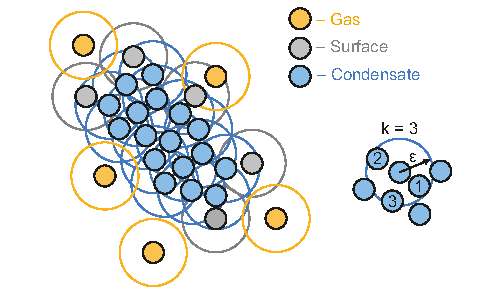
\includegraphics[width=140mm]{kepsilon.pdf}
    \caption{Принцип работы алгоритма кластеризации DBSCAN для случая $k = 3$.
    Синие точки являются основными точками (конденсатом), поскольку область с радиусом $\varepsilon$, окружающая эти точки, содержит по меньшей мере трех соседей (не считая саму точку).
    Серые точки не имеют в своей $\varepsilon$~-~окрестности трех соседей, но имеют покрайней мере одну основную точку (частицу конденсата).
    Такие точки относятся к поверхности.
    У ораневых точек в своей $\varepsilon$~-~окрестности нет ни одной основной точки, поэтому они считаются частицами газа.}
    \label{kepsilon}
\end{figure}

Важным вопросом применения данного алгоритма является выбор оптимальных значений параметров $\varepsilon$ и $k$.
В качестве функции расстояния мы используем норму Евклидова пространства, но выбор $\varepsilon$ и $k$ не так очевиден.

В задачах классификации выбор значения $\varepsilon$ часто выполняется автоматически и зависит только от $k$.
Для каждой точки данных вычисляется расстояние до самой дальней из $k$ ближайших точек.
Полученные расстояния сортируются.
На графике зависимости данного расстояния от индекса массива отсортированных точек наблюдается точка перегиба, которая определяет оптимальное значение параметра $\varepsilon$.
Наиболее эффективным способом получения такой точки является нахождение точки, наиболее удаленной от прямой, соединяющей минимальное и максимальное значение расстояния.
Выбор оптимальных параметров иллюстрируется на рисунке~\ref{epsilon_k}.

Обнаружено, что для рассматривоемой физической задачи данный метод также подходит, поэтому единственным свободным параметром в используемом алгоритме остается значение $k$, которое имеет смысл минимального значения размера кластера, и как будет показано далее, может быть взято в большом диапазоне значений, а малое изменение данного параметра слабо влияет на результат классификации, что делает работу выбранного метода более стабильной.
Пример кластеризации системы частиц после применения алгоритма DBSCAN представлен на рисунке \ref{DBSCAN-Illustr}(a).

\begin{figure}[!t]
    \centering
    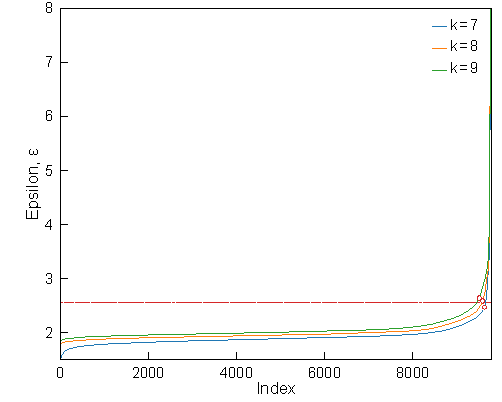
\includegraphics[width=150mm]{Figure0.pdf}
    \caption{Выбор оптимального параметра $\varepsilon$.
    Красным цветом указаны точки для различных значений параметра $k$, наиболее удаленные от линии, соединяющей начало и конец кривой расстояний.}
    \label{epsilon_k}
\end{figure}

Классификация частиц поверхности в зависимости от задачи может различаться.
При необходимости отнесения к поверхности минимального количества частиц поверхностью считаются только те частицы, которые относятся к конденсату, не будучи основными (по условию k-NN < k).
Данное выделение поверхности представлено на рисунке~\ref{DBSCAN-Illustr}(b).
Однако при необходимости выделения поверхности, полностью ограничивающей кластер, может быть применен алгоритм выделения поверхности.
Алгоритм выделения поверхности следующий: набору точек можно присвоить многоугольник с помощью набора кругов определенного радиуса, для этого вокруг точек рисуется произвольная форма, у которой удаляется как можно большая часть, используя круги определенного радиуса.
Малый радиус означает, что можно удалить больше частиц, больший радиус -- меньшее <<удаление>>.
Т.е. малый радиус создает плотную обрезанную форму, тогда как бесконечный радиус воссоздает выпуклую оболочку набора.
Точки, определенные как краевые, затем соединяются прямыми гранями, что может создать пустые области внутри набора точек.
Система, после применения данного алгоритма выделения поверхности представлена на рисунке~\ref{DBSCAN-Illustr}(c).

\begin{figure}[!t]
    \centering
    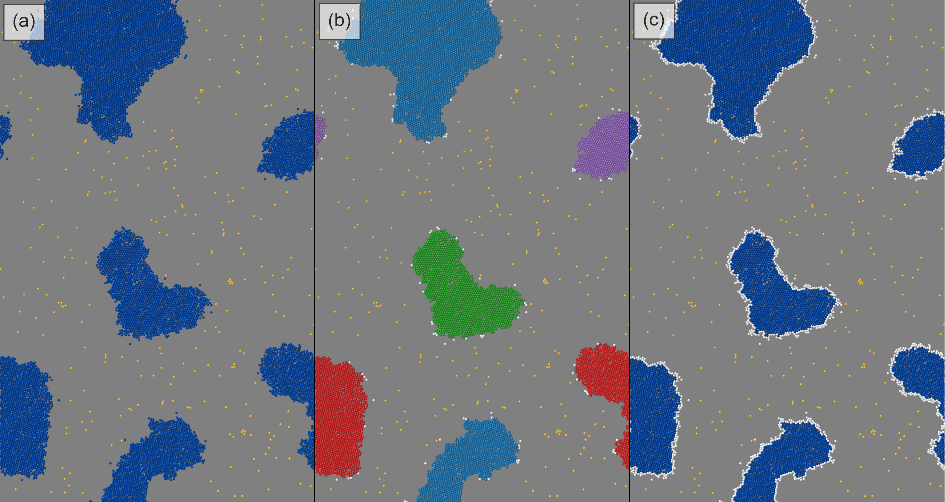
\includegraphics[width=\linewidth]{PRIMe-Figure104.pdf}
    \caption{Пример распознавания частиц в 2D системе LJ12-6. 
    (a) Результат работы метода DBSCAN (классификация частиц на конденсат и газ). 
    (b) Пример выделения частиц поверхности, по условию принадлежности к конденсату, а не к основным частицам.
    Разные кластеры раскрашены в разные цвета с учетом регулярных граничных условий. 
    (с) Пример выделения регулярной поверхности, охватывающей все частицы кластера.}
    \label{DBSCAN-Illustr}
\end{figure}

Данный метод легко обобщается на трехмерные системы.
Пример классификации частиц в трехмерном моделировании с потенциалом Леннарда-Джонса 12-6 изображен на рисунках \ref{D3_flat_layer} и \ref{D3_free_conf}.

\begin{figure}[!t]
    \centering
    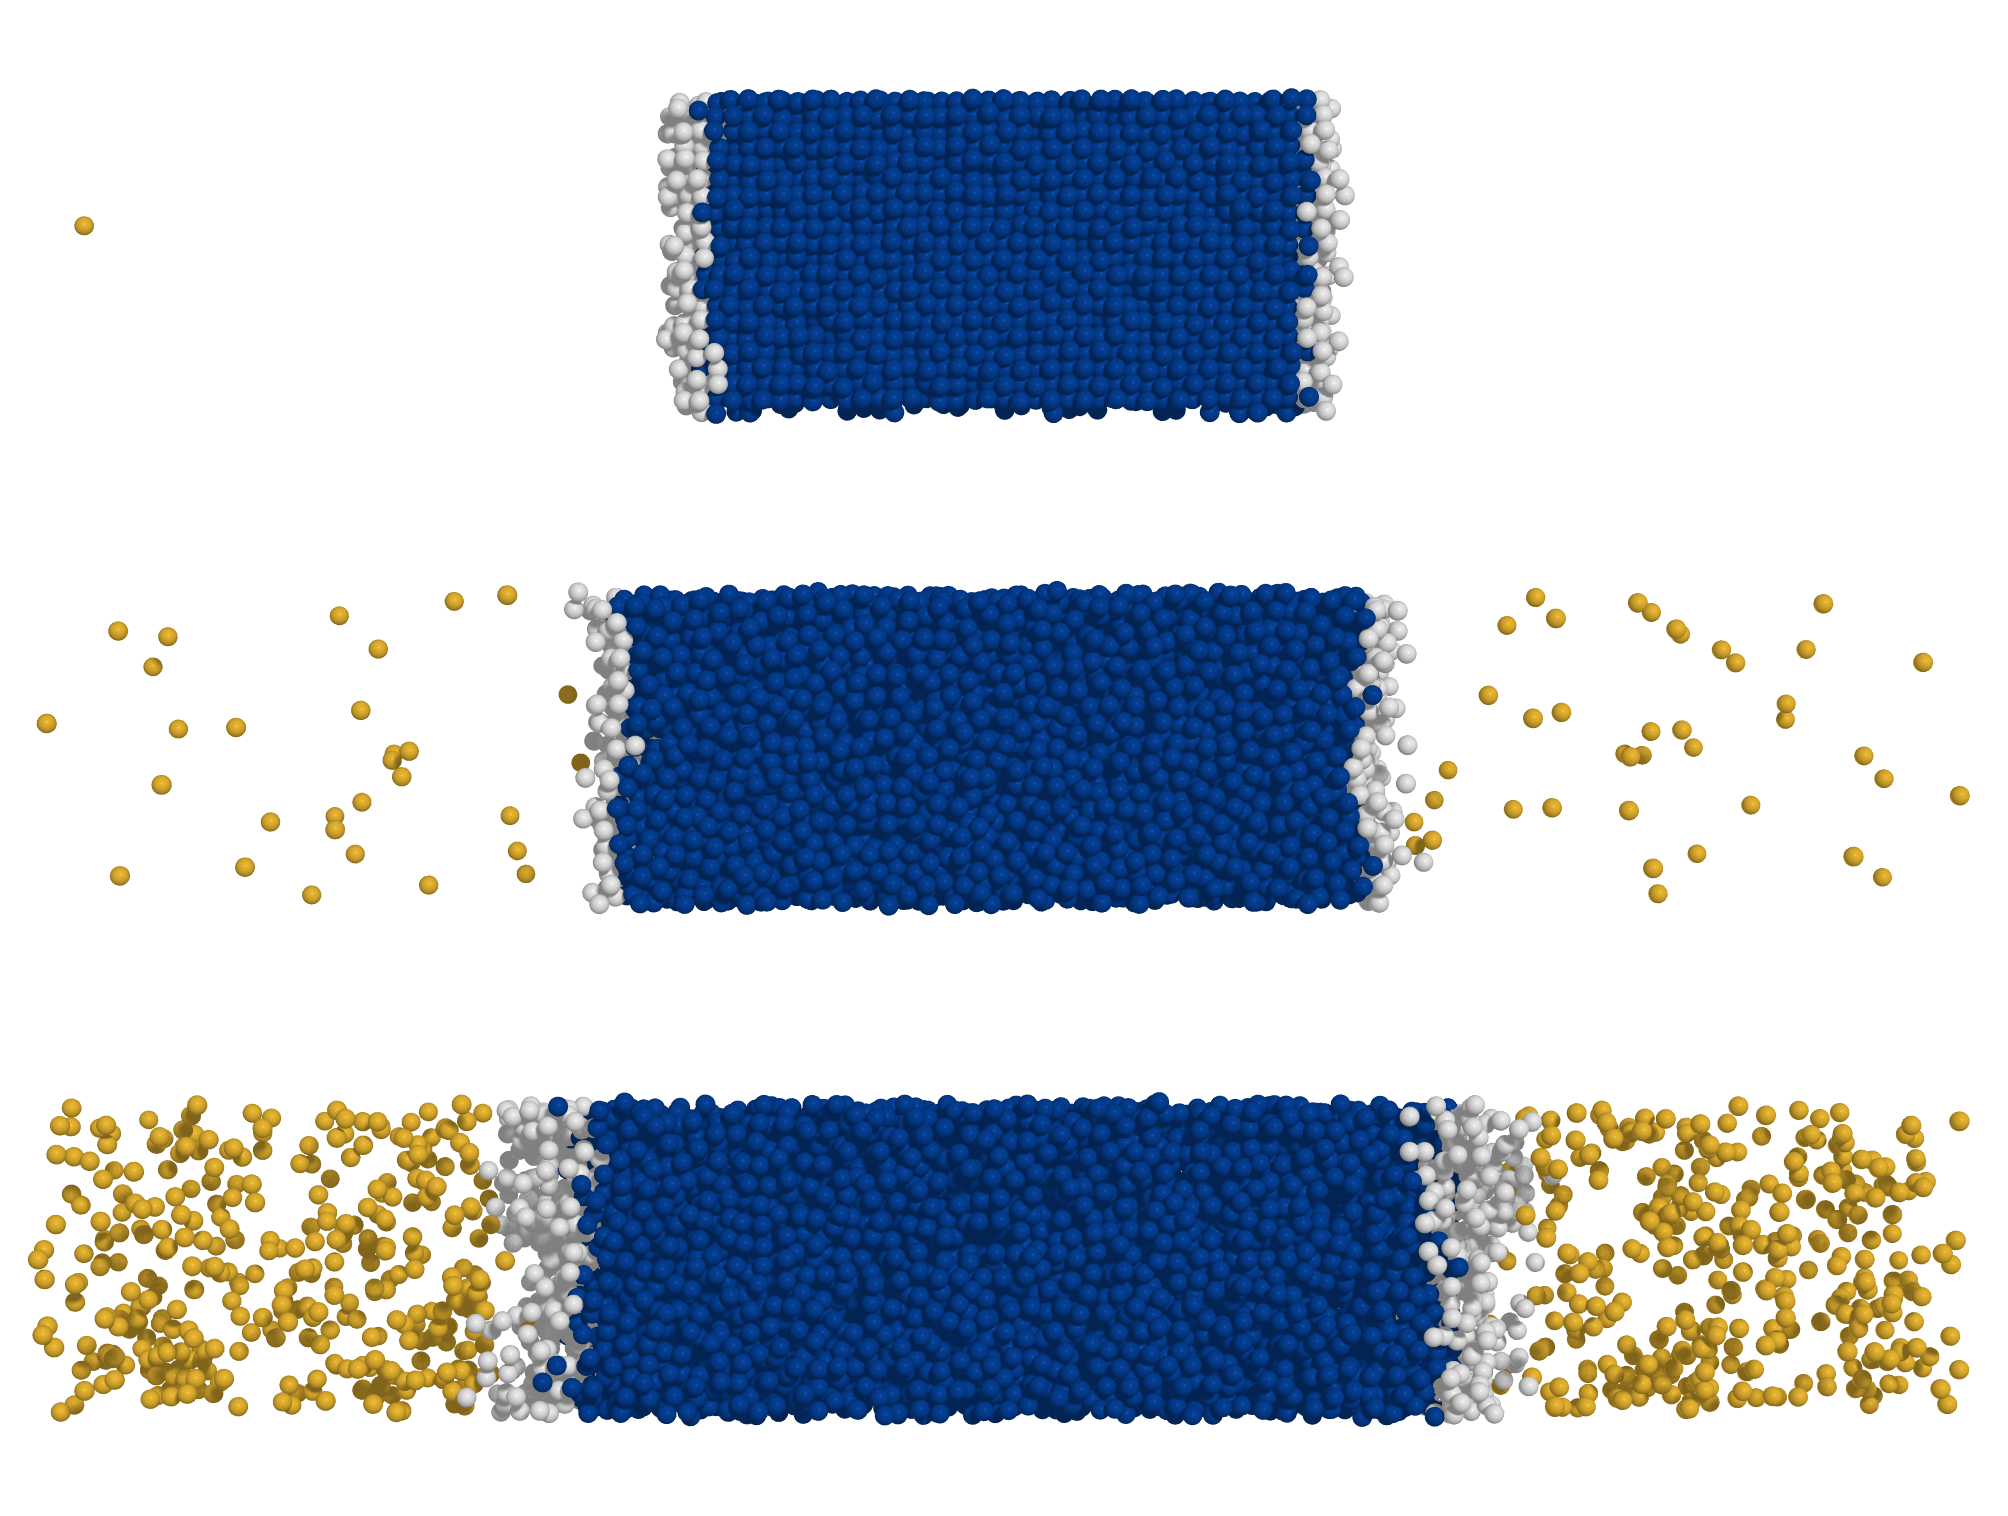
\includegraphics[width=\linewidth]{PRIMe-Figure101.png}
    \caption{Распознавание фаз методом DBSCAN в 3D системе LJ12-6 в случае плоского слоя для разных температур.}
    \label{D3_flat_layer}
\end{figure}


\begin{figure}[!t]
    \centering
    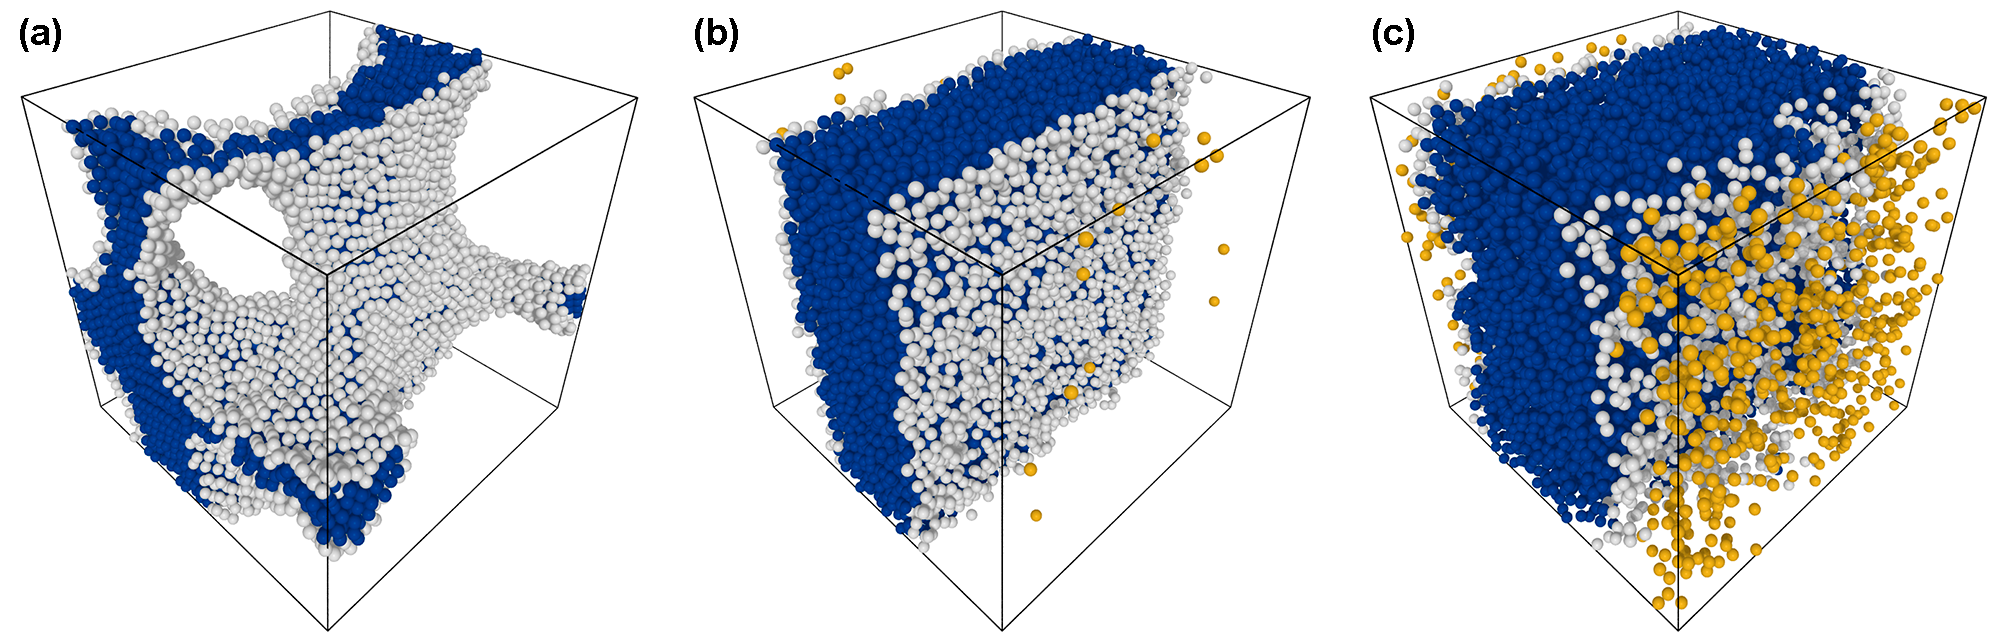
\includegraphics[width=\linewidth]{PRIMe-Figure103.png}
    \caption{Распознавание фаз для кластера произвольной формы в трехмерной системе LJ12-6 при различной температуре: (a) кластер произвольной формы при температуре ниже тройной точки; (b) система в состоянии жидкость + газ; (с) система вблизи критической точки.}
    \label{D3_free_conf}
\end{figure}



\subsection{Построение фазовых диаграмм}
\label{PRIMe-SubSecPhaseDiagram}

Новый метод классификации частиц на фазы дает возможность использовать уникальный подход к построению фазовых диаграмм, который основан на вычислении плотности подсистем, содержащих только частицы определенной фазы.
Для демонстрации работы рассматриваемого метода классификации и построения фазовых диаграмм были проведены МД-моделирования в NVT ансамбле системы частиц, взаимодействующих по обобщенному потенциалу Леннарда-Джонса (LJn-m):

\begin{equation}
U_{n-m}(r)=4 \varepsilon\left[\left(\frac{\sigma}{r}\right)^{n}-\left(\frac{\sigma}{r}\right)^{m}\right]
\label{MACR-eq1}
\end{equation}
где $\epsilon$ и $\sigma$ -- магнитуда и характерный масштаб отталкивания соответственно.
Были использованы нормированная температура $ T/ \epsilon \rightarrow T $, расстояние $ r/ \sigma \rightarrow r $ и плотность частиц $ \rho \sigma ^ 3 / m \rightarrow n$ (здесь $ m $ - масса частицы). 

В качестве примеров выступили потенциалы LJ12-4, LJ12-5, \\ LJ12-6, LJ16-6, в случае трехмерных систем, и LJ12-3, LJ12-4, LJ12-5, LJ12-6, LJ12-7, в случае двумерных.

После классификации системы на конденсат, газ и поверхность эти данные могут быть применены для различных расчетов, например, для вычисления фазовых диаграмм веществ.

Для этого случайным образом вся система разбивается на подобласти, после чего расчитываются их плотности как $\rho_i = N / V$, где $N$ -- количество частиц попавших в сферу (окружность для 2D случая) радиусом $\varepsilon$; $V$ -- объем сферы радиусом $\varepsilon$ (площадь окружности в 2D случае); $i$ -- индекс области.

Затем случайно выбранные области относятся к конденсату или газу по следующим критериям:
\begin{enumerate}
    \item Если в области $\varepsilon$ находятся только частицы конденсата и их не меньше чем $k$, то эта область является конденсатом;
    \item Если в область попали частицы поверхности, то эта область относится к поверхности и не участвует в статистике плотностей газа и конденсата;
    \item Если в область попали только газовые частицы или в области нет частиц, то эта область считается занимаемой газом.
\end{enumerate}
Затем рассчитываются плотности соответствующих областей и вычисляеется среднее значение плотности конденсата и газа.

Для расчета фазовых диаграмм вещества в координатах $\rho$-$T$ необходимо знать плотность газа и конденсата при соответствующих температурах.
Для этого в начале моделирования берется температура существенно ниже тройной точки, затем система релаксирует.
После релаксации температура системы начинает медленно линейно повышаться от температуры релаксации до закритической.
Нагревание происходит медленно, поэтому систему в каждый момент времени можно считать находящейся в состоянии термодинамического равновесия, что позволяет быстро найти для каждой температуры соответствующие плотности конденсата и газа усреднив их по нескольким соседним кадрам моделирования.

\begin{figure}[!t]
    \centering
    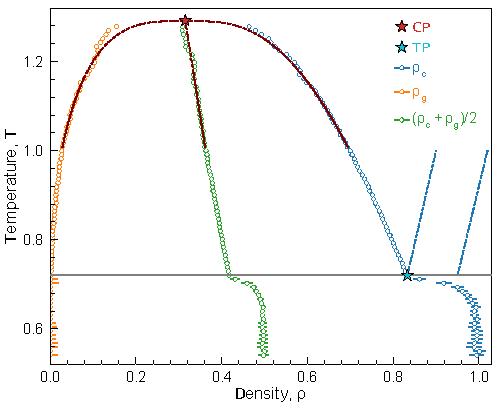
\includegraphics[width=150mm]{MACR-Figure2.pdf}
    \caption{Фазовая диаграмма системы LJ12-6, изображенной на рисунке~\ref{D3_free_conf}.
    Оранжевые и синие символы — плотности газа и конденсата, полученные путем усреднения плотности областей, соответствующих конденсату и газу.
    Зеленые символы -- медиана $\rho_m=(\rho_g+\rho_c)/2$.
    Сплошная красная линия соответствует уравнению ~\eqref{MACR-eq4}.
    Тройные и критические точки обозначены синими и красными звездочками соответственно.}
    \label{phase_diagram}
\end{figure}


\begin{table}[h!]
    \centering{
    \begin{tabular}{l|l|l|l|l|l|l}
        Потенциал & $T_{\rm CP}$ & $\rho_{\rm CP}$ & $T_{\rm TP}$ & $\rho_{\rm TP}$ & $A$ & $a$ \\ \hline
        \multicolumn{7}{c}{3D системы:} \\ \hline
        LJ12-4 & 4.416 & 0.278 & 1.500 & 0.980 & 0.578 & 0.128 \\
        LJ12-5 & 2.080 & 0.301 & 1.030 & 0.900 & 0.846 & 0.251 \\
        LJ12-6 & 1.282 & 0.308 & 0.645 & 0.865 & 1.002 & 0.385 \\
        LJ16-6 & 1.532 & 0.309 & 0.900 & 0.850 & 0.987 & 0.412 \\ \hline
        \multicolumn{7}{c}{2D системы:} \\ \hline
        LJ12-3 & 2.697 & 0.304 & 1.080 & 0.820 & 0.702 & 0.117 \\
        LJ12-4 & 1.170 & 0.350 & 0.700 & 0.792 & 0.823 & 0.150 \\
        LJ12-5 & 0.732 & 0.356 & 0.530 & 0.775 & 0.924 & 0.326 \\
        LJ12-6 & 0.517 & 0.355 & 0.405 & 0.780 & 0.982 & 1.019 \\
        LJ12-7 & 0.371 & 0.363 & 0.316 & 0.780 & 1.058 & 1.680 \\ \hline
    \end{tabular}
    }
    \caption{Значения тройных и критических точек, а также коэффициентов фитирования $A$ и $a$ из уравнений \eqref{MACR-eq4} для двумерных и трехмерных систем Леннарда-Джонса, рассматриваемых в данной работе.}
    \label{PRIMe-Table2}
\end{table}



Вблизи критической температуры вычисление плотностей газа и конденсата становится затруднительным из-за растущих флуктуаций плотности в системе.
Поэтому для более точного определения критической температуры фазовые диаграммы можно аппроксимировать следующими уравнениями~\ref{MACR-eq4}.

В трехмерии для потенциала LJ12-6 критический индекс $\beta_c = 0.325$, а в двумерии -- $\beta_c = 0.5$.
Пример построения фазовой диаграммы для трехмерной системы LJ12-6 и нахождение тройной и критической точки изображено на рисунке~\ref{phase_diagram}.

Главным достоинством такого подхода к построению фазовых диаграмм по сравнению с методами <<плоского слоя>>~\cite{10.1021/jp806127j, 10.1021/jp1117213} и термодинамическим интегрированием~\cite{10.1088/0953-8984/21/46/465104} является нечувствительность метода к форме кластеров, а также произвольное начальное и последующее расположение частиц, скорость работы алгоритма благодаря автоматизации выбора параметров и расчетов.



\subsection{Детали МД-моделирований для построения фазовых диаграмм}
\label{PRIMe-SubSecPhaseDiagramMD}



Все МД-симуляции были выполнены в ансамбле NVT (N, V и T -- количество частиц, объем системы и температура) с периодическими граничными условиями при использовании пакета моделирования LAMMPS~\cite{10.1006/jcph.1995.1039}.
Исходное состояние системы формировалось следующим образом: (i) кубический ящик (квадратный в 2D случае) моделирования заполнялся равновесным кристаллом (в данном случае ГЦК) из $N$ частиц со средней плотностью системы $\rho_a$; (ii) система релаксировала на протяжении $3 \times 10^5$ шагов при температуре $T_{start}$.
Результирующее начальное состояние для 3D системы LJ12-6 показано на рис.~\ref{D3_free_conf}(а).
Затем температура системы линейно увеличивалась от $T_{start}$ до $T_{stop}$ в течение $n_{step}$ шагов моделирования с временным шагом $\Delta t$.
Различия в моделированиях представленны в таблице \ref{MACR-Table1}.


\begin{table}[h!]
    \centering{
    \begin{tabular}{l|l|l|l|l|l|l}
        Потенциал & $\rho_a$ & $r_c$ & $T_{\rm start}$ & $T_{\rm stop}$ & $n_{step}$& $\Delta t$ \\  \hline
        \multicolumn{7}{c}{3D системы:} \\\hline
        LJ12-4 & \multirow{4}*{0.35} & 12.0 & 0.5 & 4.5 & \multirow{4}*{$5 \times 10^6$}  & \multirow{4}*{$5 \times 10 ^ {- 4}$} \\
        LJ12-5 &  & 10.0 & 0.2 & 2.5 & & \\
        LJ12-6 &  & 8.0 & 0.4 & 1.4 &  & \\
        LJ16-6 &  & 8.0 & 0.6 & 1.6 &  & \\ \hline
        \multicolumn{7}{c}{2D системы:} \\\hline
        LJ12-3 & \multirow{5}*{0.35} & 15.0 & 0.5 & 3.0 & \multirow{5}*{$7 \times 10^6$}  & \multirow{5}*{$5 \times 10 ^ {-4}$} \\
        LJ12-4 &  & 15.0 & 0.4 & 1.4 & & \\
        LJ12-5 &  & 10.0 & 0.2 & 0.9 &  & \\
        LJ12-6 &  & 8.0 & 0.35 & 0.55 &  & \\
        LJ12-7 &  & 8.0 & 0.28 & 0.4 &  & \\ \hline
    \end{tabular}
    }
    \caption{Параметры, используемые в МД-моделировании для бимодальных расчетов:
    где $\rho$ — средняя плотность системы, $r_c$ — радиус отсечки,
    $T_{start}$ и $T_{stop}$ — начальная и конечная температуры моделирования,
    $n_{step}$ — количество шагов моделирования, а
    $\Delta t$ — временной шаг.}
    \label{MACR-Table1}
\end{table}


\section{Результаты}
\label{PRIMe-SecResults}

\subsection{Результаты построения фазовых диаграмм}
\label{PRIMe-SubSecPhaseDiagramMD}

На рисунке \ref{phase_diagram}(a) и \ref{phase_diagram}(b) представленны результаты построения фазовых диаграмм для двумерия и трехмерия соответственно, расчитанные с помощью нового метода классификации частиц на фазы.
Фазовые диаграммы нормированны на температуру и плотность тройной точки, представленные в таблице \ref{PRIMe-Table2}.

Как можно заметить, представленные фазовые диаграммы имеют незначительные погрешности плотности конденсата и газа.
Данный результат показывает большую стабильность по сравнению с другими методами построения фазовых диаграмм~\cite{10.1021/jp806127j, 10.1021/jp1117213}.
Важным достоинством нового метода является то, что для расчета не требуется множество моделирований как для метода термодинамического интегрирования~\cite{10.1080/00268976.2019.1699185}. Отметим, что для рассматриваемого метода также не требуется ни системы конкретной формы, ни моделирования плоского слоя~\cite{10.1021/jp806127j, 10.1021/jp1117213}.
В таблице~\ref{PRIMe-Table3} приведено сравнение методов построения фазовых диаграмм, включая новый.



\begin{table}[h!]
    \centering{
    \begin{tabular}{l|l|l|l|l}
        Метод & Форма & 3D & Скорость & Точность \\  \hline
        Представленный метод & \checkmark & \checkmark & \checkmark & \checkmark  \\
        Метод плоского слоя~\cite{10.1021/jp806127j, 10.1021/jp1117213} & $\times$ & \checkmark & \checkmark & $\times$  \\
        Термодинамическое интегрирование~\cite{10.1080/00268976.2019.1699185} & \checkmark   & \checkmark   & $\times$   & \checkmark    \\
        Метод основанный на $R^2$-параметре~\cite{10.1021/acs.jpcc.7b09317} & \checkmark & $\times$ & \checkmark & $\times$  \\ \hline
    \end{tabular}
    }
    \caption{Сравнение различных методов построения фазовых диаграмм.
    Под 2D и 3D понимается применимость данных методов в двумерных или трехмерных системах, под скоростью -- величина затраченого времени в человеко-часах на одну точку фазовой диаграммы относительно других представленных методов, под точностью -- точность метода относительно других представленных методов.}
    \label{PRIMe-Table3}
\end{table}



\begin{figure}[!t]
    \centering
    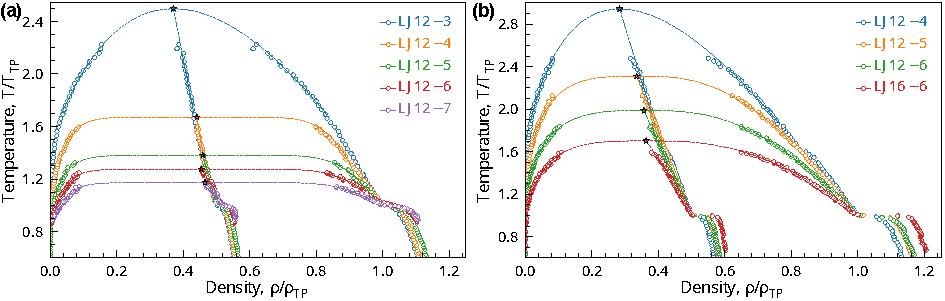
\includegraphics[width=\linewidth]{Figure11.pdf}
    \caption{Фазовые диаграммы систем с различным дальнодействием притяжения.
    (a) Фазовые диаграммы в двумерных системах.
    (b) Фазовые диаграммы в трехмерных системах.}
    \label{phase_diagram}
\end{figure}

\subsection{Тесты на устойчивость метода к плотности системы и входным параметрам}
\label{PRIMe-SubSecTests}


Для успешного применения данного алгоритма кластеризации необходимо выявить границы его применимости.
В связи с чем были проведены тесты на устойчивость метода к изменению начальной плотности системы и выбору минимального размера кластеров.

\begin{figure}[!t]
    \centering
    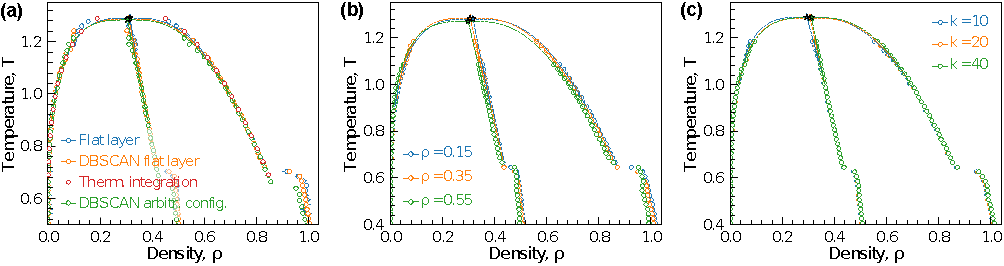
\includegraphics[width=\linewidth]{Figure10.pdf}
    \caption{\textbf{(a)} Сравнение различных методов построения фазовых диаграмм.
    Красным отмечен самый точный метод - термодинамическое интегрирование~\cite{10.1080/00268976.2019.1699185}.
             \textbf{(b)} Тест на влияние средней плотности на фазовую диаграмму системы LJ12-6 в трехмерии.
             \textbf{(c)} Тест на влияние начального параметра $k$ на фазовую диаграмму системы LJ12-6 в трехмерии.}
    \label{tests}
\end{figure}



На рисунке~\ref{tests}(b) представлен результат построения фазовых диаграмм систем с потенциалом взаимодействия LJ12-6 в трехмерии с различной начальной плотностью системы.
Примечательно, что существенное изменение плотности системы слабо влияет на расчет фазовых диаграмм и критических точек.



Кроме устойчивости к плотности системы данный алгоритм построения фазовых диаграмм также должен быть нечувствительным к изменению параметра $k$.
На рисунке~\ref{tests}(c) продемонстрирован тест на чувствительность метода к данному параметру.
Была смоделирована система с потенциалом LJ12-6 в трехмерии и применен новый метод расчета фазовых диаграмм.
Фазовые диаграммы построены с использованием различных входных параметров $k$.
Анализ результатов показывает, что изменение параметра $k$ практически не влияет на фазовую диаграмму.


Для сравнения нового метода построения фазовых диаграмм с уже существующими была проведена обработка одного моделирования новым методом и методом <<плоского слоя>>~\cite{10.1021/jp806127j, 10.1021/jp1117213}.
Кроме того, было произведено сравнение полученных результатов с фазовой диаграммой системы с произвольной начальной формой кластера.
Результаты тестов приведены на рисунке~\ref{tests}(a), где синим цветом обозначена фазовая диаграмма вычисленная методом <<плоского слоя>>, оранжевым -- фазовая диаграмма, рассчитанная новым методом распознавания фаз.
На том же моделировании, что и <<плоский слой>>, зеленым цветом показана фазовая диаграмма вычисленная новым методом, только в данном случае на моделировании с произвольным начальным расположением частиц.
Красным цветом представленны данные, расчитанные методом термодинамического интегрировния, самым точным из представленных~\cite{10.1080/00268976.2019.1699185}.

Как можно заметить, фазовая диаграмма, построенная по моделированию, содержащему плоский слой частиц, оказалась практически идентичной для разных методов.
Новый метод даёт возможность построить более плавную фазовую диаграмму и меньшую погрешность плотности кристаллической фазы.
Однако при этом новый метод, примененный к системе с произвольным расположением частиц, дает несколько отличный результат от методов, примененных к плоскому слою частиц.
Это явление вызвано тем, что <<плоский слой>> частиц более стабильный и может находится в состоянии перегретого кристалла, в то время как на кластерах произвольной формы зародыши плавления начинают появляться при меньшей температуре.
Данный факт делает метод <<плоского слоя>> не таким универсальным, как новый метод классификации, основанный на DBSCAN, так как результирующие фазовые диаграммы полученные методом <<плоского слоя>> имеют завышенную тройную точку, в отличии от нового метода, который способен строить фазовую диаграмму для систем с произвольной формой.


\section{Изучения скорости нуклеации в переохлажденных системах}
\label{PRIMe-SecNucleation}

\begin{figure}[!t]
    \centering
    \includegraphics[width=\linewidth]{Otchet}
    \caption{Процесс зарождения и роста кластеров в переохлажденной системе частиц взаимодействующих посредством потенциала Леннарда-Джонса.}
    \label{otchet}
\end{figure}


\begin{figure}[!t]
    \centering
    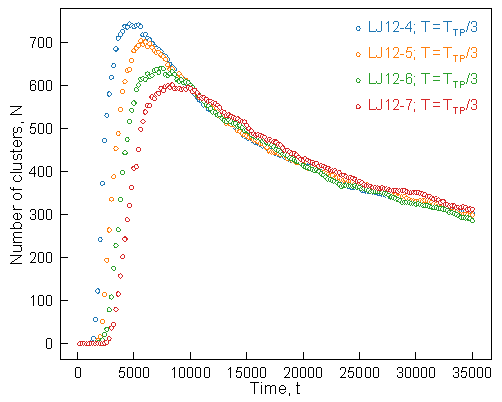
\includegraphics[width=150mm]{countCluster}
    \caption{Зависимость количества кластеров от времени.}
    \label{countCluster}
\end{figure}

\begin{figure}[!t]
    \centering
    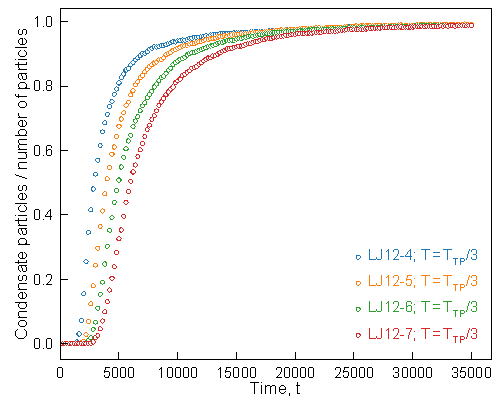
\includegraphics[width=150mm]{countParticles}
    \caption{Зависимость доли частиц, находящихся в конденсированном состоянии от времени для различных потенциалов.}
    \label{countParticles}
\end{figure}

\begin{figure}[!t]
    \centering
    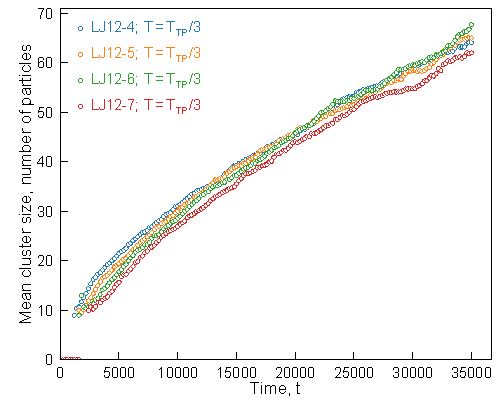
\includegraphics[width=150mm]{meanParticles}
    \caption{Зависимость среднего размера кластера от времени для систем с различным дальнодействием потенциала.}
    \label{meanParticles}
\end{figure}

Для демонстрации возможностей нового метода распознавания фаз было решено определить влияние дальнодействия потенциала на скорость нуклеации в системе с одинаковой степенью переохлаждения.

Для того, чтобы исключить влияние глубины потенциальной ямы на скорость нуклеации, был выбран нормированный потенциал из предыдущих работ~\ref{LJnm}.

При данном потенциале взаимодействия глубина остается постоянно равной единице, в то время как дальнодействие можно изменять варьируя степень притяжения $m$.

Для выяснения степени переохлаждения системы были вычислены температурные точки для двумерных систем $U_{12-4}$, $U_{12-5}$, $U_{12-6}$, $U_{12-7}$.
Значение температуры тройной точки определяется по резкому уменьшению плотности бинодали жидкость-газ.

Затем моделируются системы с равномерной плотностью распределения частиц и одинаковой степенью переохлаждения, то есть температура моделирования -- это $T = T_{TP} / a$, где в рамках нашей задачи $a = 3.0$, а $T_{TP}$ является температурой тройной точки и вычисляется на предыдущем шаге.

На рисунке~\ref{otchet} представлены снимки системы спустя разные отрезки времени после начала моделирования.
Новый алгоритм классификации на фазы позволяет наблюдать за процессами зарождения и последующего <<слипания>> кластеров.


На рисунке~\ref{countCluster} изображена временная зависимость количества кластеров в системах с различным дальнодействием притяжения. 
Видно, что дальнодействие притяжения существенно влияет на начальные этапы нуклеации, но никак не влияет на дальнейшее увеличение кластеров посредством слипания.
Существенное отличие графиков на начальном этапе объясняется тем, что дальнодействие потенциала позволяет быстрее собраться частицам в кластер нужного размера для попадания в статистику, так как кластерами в данном алгоритме считаются только те скопления частиц, которые больше критического значения, то есть $k = 9$.


На рисунке~\ref{countParticles} продемонстрирована временная зависимость доли частиц, находящихся в конденсированном состоянии.
Заметно, что скорость, с которой частицы становятся частицами кластера, зависит от дальнодействия потенциала.
Закономерно, что в случае более дальнодействующего потенциала частицы слипаются быстрее, чем при короткодействующем.


На рисунке~\ref{meanParticles} изображена зависимость среднего размера кластера от времени.
Отметим, что дальнейший рост кристаллов мало зависит от дальнодействия потенциала, а наклон зависимости среднего количества частиц одинаков для всех рассматриваемых потенциалов.


\section{Заключение главы}
\label{PRIMe-SecConclusions}

В данной главе описан новый разработанный метод распознавания фаз, основанный на алготиме кластеризации DBSCAN.
В совокупности с алгоритмом выделения поверхности новый метод позволяет с высокой точность расчитывать фазовые диаграммы систем с различной плотностью и формами кластеров.
Еще одним существенным преимуществом нового метода является его универсальность по отношению к размерности системы и нечувствительность к начальным параметрам алгоритма кластеризации.
В данной главе был также проведен сравнительный анализ различных методов построения фазовых диаграмм, среди которых новый метод является самым универсальным, сохраняя при этом точность на уровне других методов и иногда превосходя их.
Проиллюстрировано, как новый метод распознавания фаз может быть применен к переохлажденным системам частиц для анализа скорости нуклеации при различном дальнодействии притяжения.
